\documentclass{article}\usepackage[]{graphicx}\usepackage[]{color}
% maxwidth is the original width if it is less than linewidth
% otherwise use linewidth (to make sure the graphics do not exceed the margin)
\makeatletter
\def\maxwidth{ %
  \ifdim\Gin@nat@width>\linewidth
    \linewidth
  \else
    \Gin@nat@width
  \fi
}
\makeatother

\definecolor{fgcolor}{rgb}{0.345, 0.345, 0.345}
\newcommand{\hlnum}[1]{\textcolor[rgb]{0.686,0.059,0.569}{#1}}%
\newcommand{\hlstr}[1]{\textcolor[rgb]{0.192,0.494,0.8}{#1}}%
\newcommand{\hlcom}[1]{\textcolor[rgb]{0.678,0.584,0.686}{\textit{#1}}}%
\newcommand{\hlopt}[1]{\textcolor[rgb]{0,0,0}{#1}}%
\newcommand{\hlstd}[1]{\textcolor[rgb]{0.345,0.345,0.345}{#1}}%
\newcommand{\hlkwa}[1]{\textcolor[rgb]{0.161,0.373,0.58}{\textbf{#1}}}%
\newcommand{\hlkwb}[1]{\textcolor[rgb]{0.69,0.353,0.396}{#1}}%
\newcommand{\hlkwc}[1]{\textcolor[rgb]{0.333,0.667,0.333}{#1}}%
\newcommand{\hlkwd}[1]{\textcolor[rgb]{0.737,0.353,0.396}{\textbf{#1}}}%
\let\hlipl\hlkwb

\usepackage{framed}
\makeatletter
\newenvironment{kframe}{%
 \def\at@end@of@kframe{}%
 \ifinner\ifhmode%
  \def\at@end@of@kframe{\end{minipage}}%
  \begin{minipage}{\columnwidth}%
 \fi\fi%
 \def\FrameCommand##1{\hskip\@totalleftmargin \hskip-\fboxsep
 \colorbox{shadecolor}{##1}\hskip-\fboxsep
     % There is no \\@totalrightmargin, so:
     \hskip-\linewidth \hskip-\@totalleftmargin \hskip\columnwidth}%
 \MakeFramed {\advance\hsize-\width
   \@totalleftmargin\z@ \linewidth\hsize
   \@setminipage}}%
 {\par\unskip\endMakeFramed%
 \at@end@of@kframe}
\makeatother

\definecolor{shadecolor}{rgb}{.97, .97, .97}
\definecolor{messagecolor}{rgb}{0, 0, 0}
\definecolor{warningcolor}{rgb}{1, 0, 1}
\definecolor{errorcolor}{rgb}{1, 0, 0}
\newenvironment{knitrout}{}{} % an empty environment to be redefined in TeX

\usepackage{alltt}

\usepackage{float}
\usepackage{amsmath}

% Set the margins on the page to not be so large
\addtolength{\oddsidemargin}{-.875in}
\addtolength{\evensidemargin}{-.875in}
\addtolength{\textwidth}{1.75in}
\addtolength{\topmargin}{-.875in}
\addtolength{\textheight}{1.75in}

% Take off page numbering
\pagenumbering{gobble}
\IfFileExists{upquote.sty}{\usepackage{upquote}}{}
\begin{document}

\title{%
4.1.1: R - Penalized Regression Methods \\
(Ridge Regression, LASSO, and Elastic Net) \\
\smallskip
\large Stat 5100: Dr. Bean
}
\date{}

\maketitle

\subsubsection*{Matrix Specification}

Up to this point in the course, we have specified models using formula notation such as: 

\begin{knitrout}
\definecolor{shadecolor}{rgb}{0.969, 0.969, 0.969}\color{fgcolor}\begin{kframe}
\begin{alltt}
\hlstd{linear_model} \hlkwb{<-} \hlkwd{lm}\hlstd{(response} \hlopt{~} \hlstd{x1} \hlopt{+} \hlstd{x2,} \hlkwc{data} \hlstd{= mydata)}
\end{alltt}
\end{kframe}
\end{knitrout}

However, there are some functions in R that require a matrix specification. This requires us to organize the explanatory variables as a matrix ($X$) (performing variable transformations beforehand) and the response variable as a vector ($y$). As an example:

\begin{knitrout}
\definecolor{shadecolor}{rgb}{0.969, 0.969, 0.969}\color{fgcolor}\begin{kframe}
\begin{alltt}
\hlcom{# Either:}
\hlstd{model} \hlkwb{<-} \hlkwd{somemodel}\hlstd{(y, X)}
\hlcom{# Or in some packages:}
\hlstd{model} \hlkwb{<-} \hlkwd{somemodel}\hlstd{(X, y)}
\end{alltt}
\end{kframe}
\end{knitrout}

In the above, the variable $X$ is a matrix in R where each column would contain our predictor variables $x_1$, $x_2$, etc. and our rows would contain the different observations. For example, $X_{i, j}$ (meaning the $i^\text{th}$ row of $X$ and the $j^\text{th}$ column of $X$) would refer to the recorded value of $x_j$ (the $j^\text{th}$ predictor variable for the the $i^\text{th}$ observation in our data.

The matrix vs formula model specification is a product of open source software: each R package software contributor requires different model inputs in order for their functions to run properly. This in mind, always be sure to study the function documentation before you start trying to use a new R package. While there are formula-based version of the penalized regression techniques, these notes use a package that requires matrix style inputs due to its ease of implementation and consistency across the three main penalized regression approaches. 

\medskip
\hrule
\medskip

\textbf{Example: } (Ridge Regression; recall Handout 2.6.1 example) A study seeks to relate (in females) amount of body fat ($Y$) to triceps skinfold thickness ($X_1$), thigh circumference ($X_2$), and midarm circumference ($X_3$).  Amount of body fat is expensive to measure, requiring immersion of person in water.  This expense motivates the desire for a predictive model based on these inexpensive predictors.

\begin{knitrout}
\definecolor{shadecolor}{rgb}{0.969, 0.969, 0.969}\color{fgcolor}\begin{kframe}
\begin{alltt}
\hlcom{# Load the data}
\hlkwd{library}\hlstd{(stat5100)}
\hlkwd{data}\hlstd{(bodyfat)}

\hlcom{# Look at the original fit along with VIF:}
\hlstd{bodyfat_lm} \hlkwb{<-} \hlkwd{lm}\hlstd{(body} \hlopt{~} \hlstd{triceps} \hlopt{+} \hlstd{thigh} \hlopt{+} \hlstd{midarm,} \hlkwc{data} \hlstd{= bodyfat)}

\hlkwd{summary}\hlstd{(bodyfat_lm)}
\end{alltt}
\begin{verbatim}
## 
## Call:
## lm(formula = body ~ triceps + thigh + midarm, data = bodyfat)
## 
## Residuals:
##     Min      1Q  Median      3Q     Max 
## -3.7263 -1.6111  0.3923  1.4656  4.1277 
## 
## Coefficients:
##             Estimate Std. Error t value Pr(>|t|)
## (Intercept)  117.085     99.782   1.173    0.258
## triceps        4.334      3.016   1.437    0.170
## thigh         -2.857      2.582  -1.106    0.285
## midarm        -2.186      1.595  -1.370    0.190
## 
## Residual standard error: 2.48 on 16 degrees of freedom
## Multiple R-squared:  0.8014,	Adjusted R-squared:  0.7641 
## F-statistic: 21.52 on 3 and 16 DF,  p-value: 7.343e-06
\end{verbatim}
\begin{alltt}
\hlcom{# VIF:}
\hlstd{olsrr}\hlopt{::}\hlkwd{ols_vif_tol}\hlstd{(bodyfat_lm)}
\end{alltt}
\begin{verbatim}
##   Variables   Tolerance      VIF
## 1   triceps 0.001410750 708.8429
## 2     thigh 0.001771971 564.3434
## 3    midarm 0.009559681 104.6060
\end{verbatim}
\begin{alltt}
\hlcom{# Try ridge regression as a remedial measure}
\hlcom{# -----------------------------------------}
\hlcom{# We use the glmnet() function inside the glmnet package to do this. Note that}
\hlcom{# instead of specifying our model using a formula (formulas in R are of the}
\hlcom{# form Y ~ X1 + X2 + X3), we create a dataframe of just our predictor variables}
\hlcom{# and a vector of our response variable.}
\hlstd{y} \hlkwb{<-} \hlstd{bodyfat}\hlopt{$}\hlstd{body}

\hlcom{# Our X must come in the form of a matrix. First we take out the "body" column}
\hlcom{# from the dataframe, and then we convert it to a matrix.}
\hlstd{X} \hlkwb{<-} \hlkwd{as.matrix}\hlstd{(}\hlkwd{subset}\hlstd{(bodyfat,} \hlkwc{select} \hlstd{=} \hlopt{-}\hlstd{body))}

\hlcom{# Ridge regression requires that we first standarize our explanatory variables. }
\hlcom{# However, the glmnet implementation does this automatically for you }
\hlcom{# within the function so we do not need to standardize prior to use. }

\hlcom{# Rather than select an optimal value of lambda using the trace plot }
\hlcom{# (see 4.1 notes), we will select an optimal value for lambda by minimizing }
\hlcom{# the 5-fold cross validated error. }
\hlkwd{set.seed}\hlstd{(}\hlnum{123}\hlstd{)} \hlcom{# Set seed for reproducibility. }
\hlstd{bodyfat_test_ridge_lm} \hlkwb{<-} \hlstd{glmnet}\hlopt{::}\hlkwd{cv.glmnet}\hlstd{(X, y,} \hlkwc{alpha} \hlstd{=} \hlnum{0}\hlstd{,} \hlkwc{nfolds} \hlstd{=} \hlnum{5}\hlstd{)}
\hlstd{bodyfat_test_ridge_lm}
\end{alltt}
\begin{verbatim}
## 
## Call:  glmnet::cv.glmnet(x = X, y = y, nfolds = 5, alpha = 0) 
## 
## Measure: Mean-Squared Error 
## 
##     Lambda Index Measure    SE Nonzero
## min  0.437   100   7.247 1.195       3
## 1se  2.125    83   8.434 2.337       3
\end{verbatim}
\end{kframe}
\end{knitrout}

Here let's pick $\lambda = 0.437$ based upon the above output.

\begin{knitrout}
\definecolor{shadecolor}{rgb}{0.969, 0.969, 0.969}\color{fgcolor}\begin{kframe}
\begin{alltt}
\hlcom{# Use the non-cv version to actually create a model that we can use and predict with.}
\hlstd{bodyfat_ridge_lm} \hlkwb{<-} \hlstd{glmnet}\hlopt{::}\hlkwd{glmnet}\hlstd{(X, y,} \hlkwc{alpha} \hlstd{=} \hlnum{0}\hlstd{,} \hlkwc{lambda} \hlstd{=} \hlnum{0.437}\hlstd{)}
\hlcom{# Look at coefficients}
\hlstd{bodyfat_ridge_lm}\hlopt{$}\hlstd{beta}
\end{alltt}
\begin{verbatim}
## 3 x 1 sparse Matrix of class "dgCMatrix"
##                 s0
## triceps  0.4379510
## thigh    0.4369632
## midarm  -0.1193229
\end{verbatim}
\begin{alltt}
\hlcom{# Store our coefficients. You could do this by manually entering the numbers,}
\hlcom{# but we index them here for better automation.}
\hlstd{triceps_coef} \hlkwb{<-} \hlstd{bodyfat_ridge_lm}\hlopt{$}\hlstd{beta[}\hlnum{1}\hlstd{]}
\hlstd{thigh_coef} \hlkwb{<-} \hlstd{bodyfat_ridge_lm}\hlopt{$}\hlstd{beta[}\hlnum{2}\hlstd{]}
\hlstd{midarm_coef} \hlkwb{<-} \hlstd{bodyfat_ridge_lm}\hlopt{$}\hlstd{beta[}\hlnum{3}\hlstd{]}
\end{alltt}
\end{kframe}
\end{knitrout}

In order to get $b_0$ for the \textit{unstandardized} coefficients, we use the formula:
\[\beta_0 = \bar{Y} - \beta_1 \bar{X}_1 - \beta_2 \bar{X}_2 - \beta_3 \bar{X}_3\]

\begin{knitrout}
\definecolor{shadecolor}{rgb}{0.969, 0.969, 0.969}\color{fgcolor}\begin{kframe}
\begin{alltt}
\hlcom{# Means of various variables}
\hlkwd{mean}\hlstd{(bodyfat}\hlopt{$}\hlstd{body)}
\end{alltt}
\begin{verbatim}
## [1] 20.195
\end{verbatim}
\begin{alltt}
\hlkwd{mean}\hlstd{(bodyfat}\hlopt{$}\hlstd{triceps)}
\end{alltt}
\begin{verbatim}
## [1] 25.305
\end{verbatim}
\begin{alltt}
\hlkwd{mean}\hlstd{(bodyfat}\hlopt{$}\hlstd{thigh)}
\end{alltt}
\begin{verbatim}
## [1] 51.17
\end{verbatim}
\begin{alltt}
\hlkwd{mean}\hlstd{(bodyfat}\hlopt{$}\hlstd{midarm)}
\end{alltt}
\begin{verbatim}
## [1] 27.62
\end{verbatim}
\begin{alltt}
\hlcom{# Crunch our b0 formula:}
\hlstd{b0_estimate} \hlkwb{<-} \hlkwd{mean}\hlstd{(bodyfat}\hlopt{$}\hlstd{body)} \hlopt{-} \hlstd{(triceps_coef} \hlopt{*} \hlkwd{mean}\hlstd{(bodyfat}\hlopt{$}\hlstd{triceps))} \hlopt{-}
  \hlstd{(thigh_coef} \hlopt{*} \hlkwd{mean}\hlstd{(bodyfat}\hlopt{$}\hlstd{thigh))} \hlopt{-} \hlstd{(midarm_coef} \hlopt{*} \hlkwd{mean}\hlstd{(bodyfat}\hlopt{$}\hlstd{midarm))}
\hlstd{b0_estimate}
\end{alltt}
\begin{verbatim}
## [1] -9.95106
\end{verbatim}
\begin{alltt}
\hlcom{# Confirm that our "by hand" approach matches the intercept calculated }
\hlcom{# automatically by glmnet.  }
\hlstd{bodyfat_ridge_lm}\hlopt{$}\hlstd{a0}
\end{alltt}
\begin{verbatim}
##       s0 
## -9.95106
\end{verbatim}
\end{kframe}
\end{knitrout}

\subsubsection*{Get predicted values in ridge regression}

\begin{knitrout}
\definecolor{shadecolor}{rgb}{0.969, 0.969, 0.969}\color{fgcolor}\begin{kframe}
\begin{alltt}
\hlstd{predicted_y} \hlkwb{<-} \hlkwd{predict}\hlstd{(bodyfat_ridge_lm, X)}

\hlcom{# Plot the predicted values vs observed}
\hlkwd{plot}\hlstd{(y, predicted_y,} \hlkwc{xlab} \hlstd{=} \hlstr{"Observed Body Fat"}\hlstd{,} \hlkwc{ylab} \hlstd{=} \hlstr{"Predicted Body Fat"}\hlstd{,}
     \hlkwc{main} \hlstd{=} \hlstr{"Predicted Y vs. Observed Y in Ridge Regression"}\hlstd{)}
\end{alltt}
\end{kframe}

{\centering 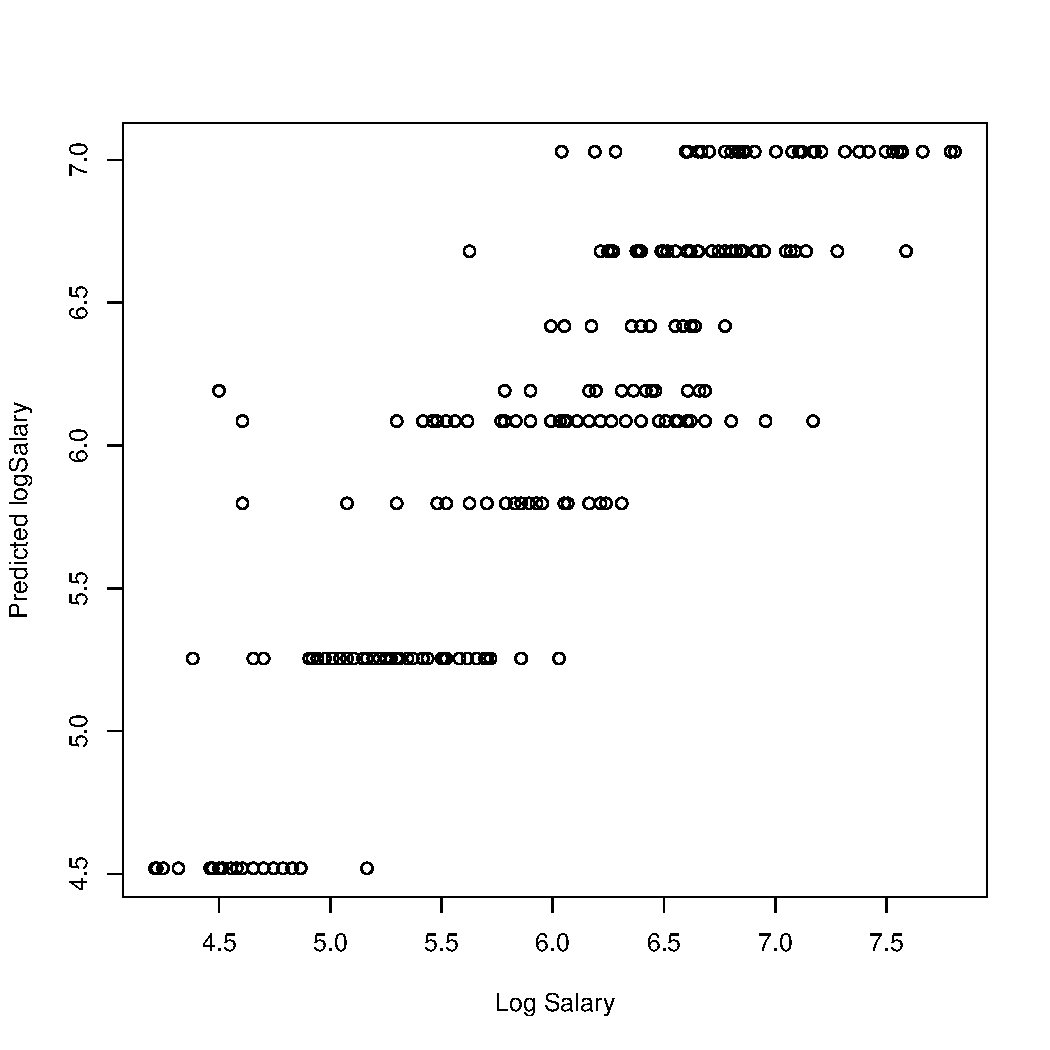
\includegraphics[width=0.6\textwidth]{figure/unnamed-chunk-6-1} 

}



\end{knitrout}

\medskip
\hrule
\medskip

\subsection*{Example 2: Baseball}

This data set (from SAS Help: the dataset has been imported into this R package) contains salary (for 1987) and performance (1986 and some career) data for 322 MLB players who played at least one game in both 1986 and 1987 seasons, excluding pitchers. How can salary be predicted from performance?

\begin{knitrout}
\definecolor{shadecolor}{rgb}{0.969, 0.969, 0.969}\color{fgcolor}\begin{kframe}
\begin{alltt}
\hlcom{# Load and take a look at the baseball dataset}
\hlkwd{data}\hlstd{(baseball)}
\hlkwd{head}\hlstd{(baseball)}
\end{alltt}
\begin{verbatim}
##                Name      Team nAtBat nHits nHome nRuns nRBI nBB YrMajor CrAtBat
## 1    Allanson, Andy Cleveland    293    66     1    30   29  14       1     293
## 2       Ashby, Alan   Houston    315    81     7    24   38  39      14    3449
## 3       Davis, Alan   Seattle    479   130    18    66   72  76       3    1624
## 4     Dawson, Andre  Montreal    496   141    20    65   78  37      11    5628
## 5 Galarraga, Andres  Montreal    321    87    10    39   42  30       2     396
## 6  Griffin, Alfredo   Oakland    594   169     4    74   51  35      11    4408
##   CrHits CrHome CrRuns CrRbi CrBB   League Division Position nOuts nAssts
## 1     66      1     30    29   14 American     East        C   446     33
## 2    835     69    321   414  375 National     West        C   632     43
## 3    457     63    224   266  263 American     West       1B   880     82
## 4   1575    225    828   838  354 National     East       RF   200     11
## 5    101     12     48    46   33 National     East       1B   805     40
## 6   1133     19    501   336  194 American     West       SS   282    421
##   nError Salary Div logSalary
## 1     20     NA  AE        NA
## 2     10  475.0  NW  6.163315
## 3     14  480.0  AW  6.173786
## 4      3  500.0  NE  6.214608
## 5      4   91.5  NE  4.516339
## 6     25  750.0  AW  6.620073
\end{verbatim}
\begin{alltt}
\hlcom{# Subset the dataset to retain only variables that are relevant for prediction}
\hlcom{# and remove all NAs prior to model input (algorithm fails if NAs are retained)}
\hlstd{baseball_sub} \hlkwb{<-} \hlkwd{subset}\hlstd{(baseball,} \hlkwc{select} \hlstd{=} \hlkwd{c}\hlstd{(logSalary, nAtBat, nHits,}
                                            \hlstd{nHome, nRuns, nRBI, nBB, YrMajor,}
                                            \hlstd{CrAtBat, CrHits, CrHome, CrRuns,}
                                            \hlstd{CrRbi, CrBB, nOuts, nAssts, nError,}
                                            \hlstd{League, Division))}

\hlstd{baseball_sub} \hlkwb{<-} \hlkwd{na.omit}\hlstd{(baseball_sub)}

\hlcom{# Take log-transformation of salary and create design matrix.}
\hlcom{# Note that this function only retains observations with no missing values }
\hlcom{# for the variables specified in the formula. We removed missing values }
\hlcom{# prior to this step in order to keep X (baseball_design) and y}
\hlcom{# (baseball_sub$logSalary) aligned. }
\hlcom{# The [, -1] omits the intercept column since glm will fit one automatically}
\hlstd{baseball_design} \hlkwb{<-} \hlkwd{model.matrix}\hlstd{(}\hlkwc{object} \hlstd{= logSalary} \hlopt{~} \hlstd{nAtBat} \hlopt{+} \hlstd{nHits} \hlopt{+} \hlstd{nHome} \hlopt{+}
                                  \hlstd{nRuns} \hlopt{+} \hlstd{nRBI} \hlopt{+} \hlstd{nBB} \hlopt{+} \hlstd{YrMajor} \hlopt{+} \hlstd{CrAtBat} \hlopt{+}
                                  \hlstd{CrHits} \hlopt{+} \hlstd{CrHome} \hlopt{+} \hlstd{CrRuns} \hlopt{+} \hlstd{CrRbi} \hlopt{+} \hlstd{CrBB} \hlopt{+}
                                  \hlstd{nOuts} \hlopt{+} \hlstd{nAssts} \hlopt{+} \hlstd{nError} \hlopt{+} \hlstd{League} \hlopt{+} \hlstd{Division,}
                                \hlkwc{data} \hlstd{= baseball_sub)[,} \hlopt{-}\hlnum{1}\hlstd{]}
\end{alltt}
\end{kframe}
\end{knitrout}

First, let's use Lasso regression:

\begin{knitrout}
\definecolor{shadecolor}{rgb}{0.969, 0.969, 0.969}\color{fgcolor}\begin{kframe}
\begin{alltt}
\hlstd{baseball_lasso_optimal} \hlkwb{<-} \hlstd{glmnet}\hlopt{::}\hlkwd{cv.glmnet}\hlstd{(baseball_design,}
                                            \hlstd{baseball_sub}\hlopt{$}\hlstd{logSalary,}
                                            \hlkwc{alpha} \hlstd{=} \hlnum{1}\hlstd{)}
\hlstd{baseball_lasso_optimal}\hlopt{$}\hlstd{lambda.min}
\end{alltt}
\begin{verbatim}
## [1] 0.01525366
\end{verbatim}
\begin{alltt}
\hlcom{# Pick optimal lambda from the above}
\hlstd{baseball_lasso} \hlkwb{<-} \hlstd{glmnet}\hlopt{::}\hlkwd{glmnet}\hlstd{(baseball_design,}
                                 \hlstd{baseball_sub}\hlopt{$}\hlstd{logSalary,}
                                 \hlkwc{alpha} \hlstd{=} \hlnum{1}\hlstd{,}
                                 \hlkwc{lambda} \hlstd{= baseball_lasso_optimal}\hlopt{$}\hlstd{lambda.min)}
\hlstd{baseball_lasso}\hlopt{$}\hlstd{beta}
\end{alltt}
\begin{verbatim}
## 18 x 1 sparse Matrix of class "dgCMatrix"
##                           s0
## nAtBat          .           
## nHits           0.0067888515
## nHome           0.0025273020
## nRuns           .           
## nRBI            .           
## nBB             0.0057078209
## YrMajor         0.0653074206
## CrAtBat         .           
## CrHits          0.0002562012
## CrHome          .           
## CrRuns          .           
## CrRbi           .           
## CrBB            .           
## nOuts           0.0001707651
## nAssts          .           
## nError         -0.0060889931
## LeagueNational  0.0645659173
## DivisionWest   -0.1255002632
\end{verbatim}
\begin{alltt}
\hlstd{baseball_lasso}\hlopt{$}\hlstd{a0}
\end{alltt}
\begin{verbatim}
##       s0 
## 4.283545
\end{verbatim}
\end{kframe}
\end{knitrout}

Now, let's show an example with elastic net regression. This is specified by using some alpha between 0 and 1. For simplicity, we we will pick $\alpha = 0.5$.

\begin{knitrout}
\definecolor{shadecolor}{rgb}{0.969, 0.969, 0.969}\color{fgcolor}\begin{kframe}
\begin{alltt}
\hlstd{baseball_elnet_optimal} \hlkwb{<-} \hlstd{glmnet}\hlopt{::}\hlkwd{cv.glmnet}\hlstd{(baseball_design,}
                                            \hlstd{baseball_sub}\hlopt{$}\hlstd{logSalary,}
                                            \hlkwc{alpha} \hlstd{=} \hlnum{0.5}\hlstd{)}
\hlstd{baseball_elnet_optimal}\hlopt{$}\hlstd{lambda.min}
\end{alltt}
\begin{verbatim}
## [1] 0.02532772
\end{verbatim}
\begin{alltt}
\hlcom{# Pick optimal lambda from the above}
\hlstd{baseball_elnet} \hlkwb{<-} \hlstd{glmnet}\hlopt{::}\hlkwd{glmnet}\hlstd{(baseball_design,}
                                 \hlstd{baseball_sub}\hlopt{$}\hlstd{logSalary,}
                                 \hlkwc{alpha} \hlstd{=} \hlnum{0.5}\hlstd{,}
                                 \hlkwc{lambda} \hlstd{= baseball_elnet_optimal}\hlopt{$}\hlstd{lambda.min)}

\hlcom{# Obtain beta estimates (including intercept)}
\hlstd{baseball_elnet}\hlopt{$}\hlstd{beta}
\end{alltt}
\begin{verbatim}
## 18 x 1 sparse Matrix of class "dgCMatrix"
##                           s0
## nAtBat          .           
## nHits           6.406212e-03
## nHome           2.546061e-03
## nRuns           5.455873e-04
## nRBI            6.043526e-05
## nBB             5.554989e-03
## YrMajor         6.114898e-02
## CrAtBat         1.438093e-05
## CrHits          2.344433e-04
## CrHome          .           
## CrRuns          3.177752e-06
## CrRbi           .           
## CrBB            .           
## nOuts           1.798556e-04
## nAssts          .           
## nError         -6.376027e-03
## LeagueNational  6.945671e-02
## DivisionWest   -1.287318e-01
\end{verbatim}
\begin{alltt}
\hlstd{baseball_elnet}\hlopt{$}\hlstd{a0}
\end{alltt}
\begin{verbatim}
##       s0 
## 4.303893
\end{verbatim}
\end{kframe}
\end{knitrout}


\end{document}
